% !TeX root=../main.tex

\chapter{مقدمه}
% دستور زیر باعث عدم‌نمایش شماره صفحه در اولین صفحهٔ این فصل می‌شود.
\thispagestyle{empty}
\section{پیشگفتار}
یک سیستمِ احراز هویت به‌وسیله چهره را در نظر بگیرید که کاربر در مقابل دوربین قرار‌گرفته و سیستم از طریق تایید مشخصات چهره، به او اجازه دسترسی می‌دهد. حال فرض کنید کاربر غیر‌مجاز تصویر کاربرِ قبلاً تایید شده در سیستم را روی کاغذ چاپ کند و کاغذ را در مقابلِ دوربینِ سیستم قرار دهد. در این صورت کاربر غیر‌مجاز می‌تواند خود را به‌جای کاربر مجاز به سیستم بشناساند و به اطلاعات محرمانه فرد دیگری، به کمک تنها یک تصویر چاپ‌شده، دسترسی پیدا کند. این یک مثال ساده برای تداعی مشکل امنیتی سیستم‌های احراز اصالت با چهره است.

هر چه محرمانگی و اهمیت اطلاعات ذخیره‌شده درون سیستم بیشتر باشد، مشکل امنیتی ذکر‌شده توجه بیشتری می‌طلبد. برای مثال فرض کنید سیستم مزبور به اطلاعات حساب بانکی یا اوراق بهادار یا داده‌های محرمانه یک شرکت تجاری مرتبط باشد؛ در این صورت تمامی این اطلاعات حیاتی در معرض خطر آسیب‌پذیری فرآیند تشخیص و تایید چهره خواهد بود.

این مشکل امنیتی موجب پیدایش زمینه‌ای از تحقیقات در دانشگاه و صنعت شده است که در ادبیات موضوع «جلوگیری از تقلب برای احراز هویت مبتنی بر تشخیص چهره
\LTRfootnote{Anti-spoofing for authentication based on face recognition}
» نام دارد. در این عنوان، قسمت احراز هویت مبتنی بر تشخیص چهره در‌واقع شاخه‌ای از زیست‌سنجی
%\href{Biometric}{}
\LTRfootnote{Biometric}
   است و قسمت جلوگیری از تقلب، به مسائل امنیتی کار می‌پردازد.
هدف از زیست‌سنجی، تشخیص خودکارِ افراد بر اساس ویژگی‌های زیست‌شناختی و یا رفتار اشخاص است. برای مثال چهره، عنبیه، اثر انگشت، صدا و طرز راه رفتن نمونه از ویژگی‌هایی است که هر فرد را به‌صورت منحصراً از فرد دیگر تمیز می‌دهد.  تأکید زیست‌سنجی بر «خودکار بودن» فرآیند تشخیص فرد است؛ به همین دلیل لازم است که دخالت انسان در این فرآیند حداقل شود و سیستم به‌صورت غیر نظارتی
\LTRfootnote{Unsupervised}
 فرد را تشخیص دهد.
 
در میان شاخصه‌های ذکر‌شده برای کاربرد زیست‌سنجی، استفاده از چهره اهمیت خاصی دارد. روش‌های بینایی ماشین برای تشخیص چهره سابقه طولانی دارند و به‌تازگی راه‌حل‌های استفاده از هوش مصنوعی، تشخیص چهره را دقیق‌تر و متداول‌تر کرده است. از طرفی چهره در مقایسه با اثر انگشت یا صدا و... نمایانگر آشناتر برای شناسایی یک فرد است. این ویژگی‌های چهره چه در ابزار شناسایی چه در قرابت استفاده، موجب شده است تشخیص چهره، کاربردهای دیگری نظیر پزشکی قانونی، دوربین‌های مداربسته، اجازه کنترل و دسترسی به سیستم، و دولت و تجارت الکترونیک داشته باشد.

این کاربرد گسترده و رشد استفاده از چهره در سیستم‌ها، مسائل امنیتی را نیز به همراه دارد. فرد مهاجم به‌راحتی و با هزینه‌ی کمی می‌تواند تصویر فرد مورد‌نظر خود را از طریق شبکه‌های اجتماعی یا تصویر‌برداری از فاصله‌ی دور به‌دست آورد و اقدامات لازم برای حمله را به عمل آورد.

این نوع حمله با ابزارهای مختلفی می‌تواند صورت بگیرد. برای مثال مهاجم می‌تواند تصویر فرد هدف را روی کاغذ چاپ کند، یا از یک فیلم یا تصویر ذخیره‌شده در نمایشگر دیجیتال استفاده کند. همچنین با استفاده از گریم یا ماسک می‌تواند چهره خود را شبیه به چهره فرد هدف کند. در میان انواع حمله ذکر شده استفاده از چاپ تصویر و استفاده از نمایشگر دیجیتال متداول‌تر است. استفاده از ماسک به دلیل هزینه بالا و سختی اجرا، چندان متداول نیست.

 با توجه به اهمیت موضوع و نگرانی در مورد امنیت سیستم‌های احراز هویت مبتنی بر تشخیص چهره، تحقیقات فراوانی در دانشگاه برای فائق آمدن بر این چالش انجام‌شده است. که دامنه وسیعی از روش‌های مبتنی بر بینایی ماشین کلاسیک و روش‌های جدیدتر مبتنی بر هوش مصنوعی و یادگیری عمیق را شامل می‌شود.

این چالش امنیتی می‌تواند از دید یک مسئله‌ی بینایی ماشین تعریف شود؛ به‌گونه‌ای که ورودی مسئله، تصویر از چهره یک فرد است و خروجی سیستم، یک برچسب چهره واقعی یا تقلبی است. دقت الگوریتم برای اعلام این برچسب‌گذاری، سهم مهمی در امینت کلی سیستم خواهد داشت. در برخی از روش‌ها از اطلاعات بیشتری نظیر حس‌گر حرارتی و یا مادون‌قرمز در کنار تصویر استفاده می‌شود اما این امر موجب افزایش هزینه خواهد شد. همچنین الگوریتم‌ها بر اساس استفاده از تنها یک تصویر یا یک دنباله ویدیویی نیز قابل‌تقسیم هستند.


با‌وجود تلاش‌های تحقیقاتی در این زمینه که بیش از یک دهه قدمت دارد همچنان مسئله کشف تقلب در تشخیص چهره یک مسئله چالشی می‌باشد. یکی از دلایل چالشی بودن آن، خلاقیت فرد مهاجم برای اعمال حمله جدید است؛ به‌گونه‌ای که این  حمله جدید قبلاً در داده‌های مورد‌استفاده برای توسعه الگوریتم وجود نداشته باشد. یک چالش دیگر تفاوت کیفیت و رزولوشن ابزارهای حمله، نظیر صفحه‌نمایش و کاغذ چاپ‌شده است. این مسئله زمانی بغرنج‌تر می‌شود که حتی برای کاربر انسانی نیز تمیز چهره واقعی و تقلبی دشوار خواهد شد. برای مثال در شکل 
\ref{fig:realandfake}
یکی از تصاویر تقلبی و دیگری واقعی است. همان‌طور که مشاهده می‌شود تشخیص چهره واقعی از تقلبی به‌آسانی میسر نیست.


\begin{figure}[ht]
	\centerline{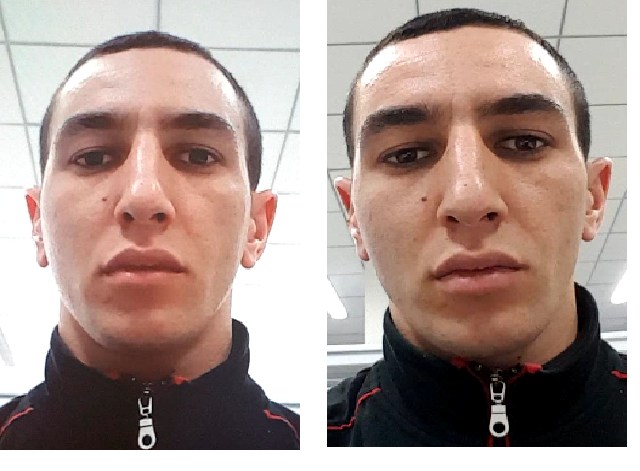
\includegraphics[width=0.7\linewidth]{realAndFakeEx}}
	\caption{نمونه‌ای از تصاویر واقعی و تقلبی در حوزه چهره \cite{boulkenafet2017oulu}}
	\label{fig:realandfake}
\end{figure}

\section{اهداف}
در این پایان‌نامه برای کشف تقلب در تصویر چهره، تمرکز بر روش‌هایی است که تنها از یک تصویر رنگی به‌جای دنباله ویدیویی یا اطلاعات اضافی نظیر حس‌گر حرارتی و مادون‌قرمز، به‌عنوان ورودی استفاده می‌شود. این رویکرد موجب کاهش هزینه سیستم و قابل‌استفاده بودن بیشتر خواهد شد. همچنین از انواع حمله‌های مختلف موجود، تنها موارد چاپ روی کاغذ و بازپخش ویدیو بررسی می‌گردد. با آن‌که حمله‌های دیگری نظیر استفاده از ماسک سه‌بعدی نیز وجود دارد اما اعمال چنین حمله‌هایی هزینه‌بر و دشوارتر از‌نظر اجرا است. بنابراین توجه پایان‌نامه روی حملاتی است که متداول‌تر و بیشتر قابل‌اجرا است. 

در این پایان‌نامه با ترکیب روش کلاسیک بینایی ماشین و روش‌های جدید یادگیری عمیق ساختاری برای طبقه‌بندی دقیق‌تر ارائه‌شده است. این ساختار شامل یک عملگر جدید است که از عملگر 
\lr{LBP} 
کلاسیک الهام گرفته‌شده است، با این تفاوت که این عملگر همانند عملگر کانولوشن در شبکه‌های عمیق دارای پارامتر برای یادگیری عملگر بهینه با توجه به داده‌های ورودی است. 
همچنین دو تابع هزینه جدید ارائه‌شده است. تابع هزینه اول با افزودن یک حاشیه به طبقه‌بندی موجب می‌شود ویژگی‌های دو کلاس با‌فاصله از یک‌دیگر قرار بگیرند که موجب افزایش دقت رو داده‌های دیده نشده می‌گردد. تابع هزینه دوم بر اساس شناسه اشخاص مختلف موجود در دیتاست توسعه داده‌شده است و موجب می‌شود که شبکه عصبی تمرکز بیشتری روی ویژگی‌های تقلب موجود در چهره داشته باشد و به ویژگی‌های ظاهری افراد توجه نکند. که این موجب افزایش قابلیت تعمیم‌پذیری شبکه روی داده‌های آزمون دیده نشده می‌شود.
\section{دستاورد‌های پژوهش}
در این پایان‌نامه، پس از بیان روش پیشنهادی به‌صورت ریاضی با آزمایش‌های مختلف روی دیتاست‌های در دسترس و محاسبه نرخ خطای استاندارد در این حوزه، نشان داده می‌شود روش ارائه‌شده شامل عملگر تحلیل ریزبافت و تابع هزینه جدید موجب افزایش دقت طبقه‌بندی و تعمیم‌پذیری آن می‌شود. قسمت‌های مختلف روش پیشنهادی هر‌کدام به‌صورت مجزا، ابتدا روی یک دیتاست کوچک ارزیابی شده‌است و اثر‌بخشی هر قسمت بررسی‌شده است. سپس تمام روش پیشنهادی روی دیتاست‌های بزرگ‌تر پیاده شده و معیار خطا با مقادیر به‌دست آمده در برخی از پژوهش‌های مهم در این حوزه مقایسه شده است. این مقایسه نشان می‌دهد روش پیشنهادی به نتایج رقابتی با نتایج این پژوهش‌ها می‌رسد. همچنین در انتها مقایسه‌ای بین هزینه‌ی محاسباتی روش ارائه‌شده با روش‌های قبلی انجام شده است که نشان می‌دهد روش پیشنهادی در عین داشتن دقت مناسب، توان محاسباتی کمتری نیاز دارد.

همچنین برای پیاده‌سازی، برنامه‌نویسی به زبان پایتون انجام شده است و ملاحظات پیاده‌سازی و چالش‌های مربوط به آن، توضیح و تفسیر شده است. علاوه بر این، برای کار کردن با داده‌های ویدیویی و استفاده از آن در شبکه‌هایی که ورودی تصویر دارند، الگوریتمی ارائه شده است که روند آموزش شبکه را تسریع ببخشد. کدهای مرتبط با برنامه در یک مخزن گیت‌هاب
\LTRfootnote{\href{https://github.com/meysamshahbazi/fas}{https://github.com/meysamshahbazi/fas}}
 به‌صورت متن‌باز منتشر شده است. برنامه به‌گونه‌ای نوشته شده است که نتایج آن قابل بازتولید باشد.
\section{ساختار پایان‌نامه}
در فصل دو، ابتدا مروری بر پژوهش‌های انجام‌شده در حوزه کشف تقلب انجام می‌شود. تحقیقات انجام‌شده در این حوزه بسیار وسیع است و تنها به مرور روش‌هایی که اهمیت بیشتر در ادبیات موضوع و روش‌هایی که رویکرد مشابهی با این پایان‌نامه داشته‌اند پرداخته می‌شود. در فصل سه، روش پیشنهادی به‌صورت مبانی نظری گفته می‌شود و در فصل چهار، ابتدا ملاحظات پیاده‌سازی روش ارائه‌شده بیان می‌گردد و سپس با استفاده از معیارهای ارزیابی متداول در این حوزه، به بررسی دقت روش پیشنهادی پرداخته می‌شود. فصل آخر به نتیجه‌گیری و بحث در مورد روش پیشنهادی می‌پردازد.


